\documentclass[prb,preprint]{revtex4-1} 
\raggedbottom
\usepackage{amsmath}
\usepackage{amsfonts}
\usepackage{graphicx}

\begin{document}

\section{Results And Analysis for Frank-Hertz Experiment}

Measurements were made of the various local current minimums which can be seen when progressively increasing the accelerating voltages, $V_a$, the the Hg gas. The voltages, and thus the average energies of the electrons at each minimum are listed in Table \ref{energies} along with the temperatures ($T$) at which they were observed. The general trend as $V_a$ is increased is displayed in Fig \ref{large} as a context to the minimums displayed in Table \ref{energies}

\begin{table}[h]
\caption{A table of $K_n$ values for each trail as labeled by their temperatures}
\begin{ruledtabular}
\begin{tabular}{c c c c c}
$T$ (C) & 157 & 165 & 186 & 190\\
\hline
$K_1\pm0.001$ eV & 7.646   & 7.518   & 7.910   & 7.918\\
$K_2\pm0.001$ eV & 11.963 & 12.577 & 12.400 & 12.552\\
$K_3\pm0.001$ eV & 17.340 & 17.757 & 17.100 & 17.269\\
$K_4\pm0.001$ eV & 22.641 & 22.933 & 21.298 & 22.037\\
$K_5\pm0.001$ eV & 28.014 & 28.298 & 26.950 & 27.041\\
$K_6\pm0.001$ eV & 33.260 & 33.263 & 31.921 & 32.065\\
$K_7\pm0.001$ eV & 39.008 & 38.862 & 37.049 & 37.078\\
\end{tabular}
\end{ruledtabular}
\label{energies}
\end{table}

\begin{figure}[h]
\centering
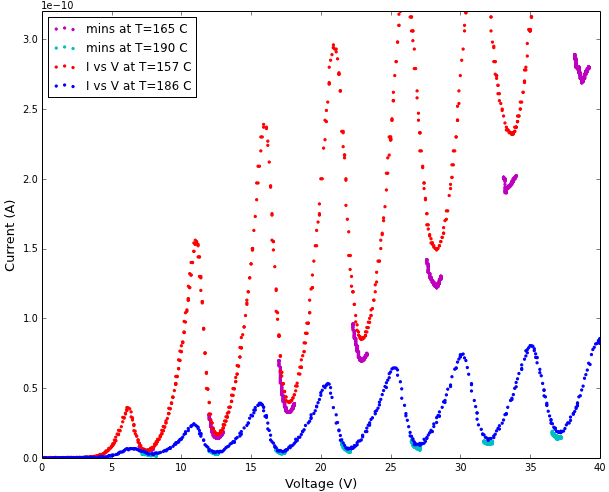
\includegraphics[width=0.7\textwidth]{large.png}
\caption{The current as a function of accelerating voltage at different $T$ values.}
\label{large}
\end{figure}

\newpage

Based upon a simple average of the differences between the voltages at each of the minimums for the two higher $T$ trials, the first excited state of mercury was determined to be $5.226\pm0.001$ eV while the contact potential difference was found to be $2.356\pm0.002$ eV. Alternatively these same values based upon the averages of the two lower $T$'s are $4.858\pm0.001$ eV for the first excited state of mercury and $3.056\pm0.002$ eV for the contact potential difference. However we are aware, through the knowledge that the mean free path of electrons changes with number density and thus $T$, that this average of all the minimum voltage differences at higher $T$'s does not accurately represent the true energy of the first excited state. Additionally we find through Fig \ref{diff} that the voltage difference increases with $n$. This leads us to believe that the most accurate measure of mercury's first excited state should arise from the voltage difference between the minimums where $n=1$ and $n=2$. As a result a more refined measured value for the first excited state can be said to be $4.562\pm0.001$ eV. However this is inconsistent with the accepted value of 4.89 eV and more closely resembles the average voltage difference at lower $T$ values.

\begin{figure}[h]
\centering
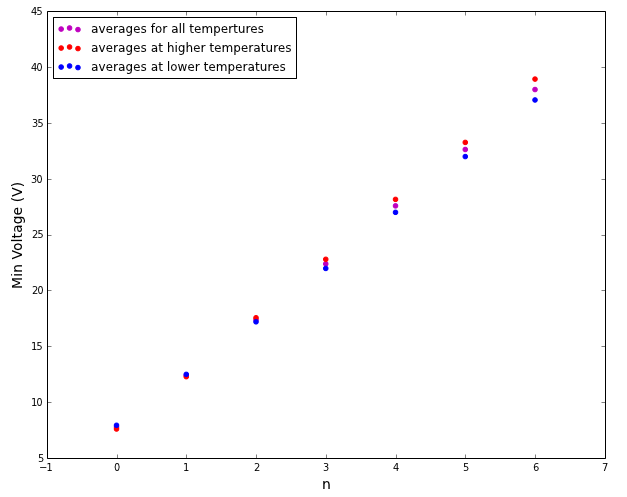
\includegraphics[width=0.65\textwidth]{diff.png}
\caption{The voltage difference at different temperatures as it varies with respect to the minimum number $n$, where $n=0$ would be the first observed minimum.}
\label{diff}
\end{figure}

\newpage

By comparing the mean free paths at different values of $T$ it becomes clear that this is why temperature created such drastic differences in our results. Table \ref{pres} presents data on the pressure ($P$) and mean free path ($\lambda$) at various $T$ values. Based on this data it's apparent that at higher $T$ the mean free path of electrons moving through the gas is significantly reduced. It can be said that the resistance of the element containing the increases with high $T$ and thus the current running through the system is reduced. This closely matches the results we find in Fig \ref{large}. As an additional piece of information, we find that by using the data in Table \ref{pres} we can determine the average number of collisions which occurred between the cathode and the anode (a distance of $\approx1$ cm) at different temperatures and thus pressures. The average number of collisions were found to be 1996$\pm40$, 18.5$\pm0.2\times10^5$, and 10.3$\pm0.2\times10^6$ collisions at the respective temperatures of 20, 157, and 186 degrees celsius.

\begin{table}[h]
\caption{The pressure and mean free path at different values of $T$}
\begin{ruledtabular}
\begin{tabular}{c c c c}
$T$ (C) & 20 & 157 & 186
\\
\hline
$P$ (kPa) & $1.79\times10^{-4}$   & 0.244   & 1.468\\
$\lambda$ (m) & $5.01\pm0.02\times10^{-4}$ & $5.394\pm0.01\times10^{-7}$ & $9.654\pm0.02\times10^{-8}$\\
\end{tabular}
\end{ruledtabular}
\label{pres}
\end{table}

The data we find in Fig \ref{large} is a perfect demonstration of the quantization of energy states in mercury. The reason being that if excitation levels in mercury were not quantized one would expect to see a continuous increase in current through the mercury filled element as accelerating voltage increase. Underlying such an observation is the fact that at low potentials, the accelerated electrons acquired only a modest amount of kinetic energy. Thus when they encounter mercury atoms in the tube, they participated in purely elastic collisions. This is due to the prediction of quantum mechanics that an atom will essentially absorb no energy until the collision energy exceeds that required to lift an electron into a higher energy state.

\section{Conclusion}

In the end our final results show that the measured value for the first excited state of Hg is $4.562\pm0.001$ eV, though this value is also inconsistent with the accepted value of 4.89 eV. Instead the accepted value more closely resembles the average voltage difference at lower $T$ values. Given this similarity to the value gleaned at lower temperatures it seems plausible that temperature played a role in giving these unexpected results. In addition to this possibility, when taking data with more resolution near the local current minimuma there appeared to be an issue in our equipment output where current values where binned to particular voltages even though no command to do so was issued. We can speculate that the data was simply binned, but the exact issue is not known and may signify a more serious problem with the data. If in fact we find that this was simply a binning problem, the fact that we took centroids of the data would motley negate any error introduced by this.

By comparing the mean free paths at different values of $T$, as are shown in Fig \ref{pres}, it's apparent that at higher $T$ the mean free path of electrons moving through the gas is significantly reduced. It can be said that the resistance of the element containing the increases with high $T$ and thus the current running through the system is reduced. We find similar results in Fig \ref{large} where the average current at higher temperatures is lower irregardless of $V_a$. Additionally, using the values shown in Table \ref{pres} we determined the average number of collisions which occurred between the cathode and the anode to be 1996$\pm40$, 18.5$\pm0.2\times10^5$, and 10.3$\pm0.2\times10^6$ collisions at the respective temperatures of 20, 157, and 186 degrees celsius.

In general, the trends we find in Fig \ref{large} are a perfect demonstration of the quantization of energy states in mercury whether or not our measurements agree with accepted value for the first excited state. The reason being that if excitation levels in mercury were not quantized one would expect to see a continuous increase in current through the mercury filled element as accelerating voltage increase. Underlying such an observation is the fact that at low potentials, the accelerated electrons acquired only a modest amount of kinetic energy. Thus when they encounter mercury atoms in the tube, they participated in purely elastic collisions. This is due to the prediction of quantum mechanics that an atom can absorb no energy until the collision energy exceeds that required to lift an electron into a higher energy state.

\end{document}
